%%%%%%%%%%%%%%%%%%%%%%%%%%%%%%%%%%%%%%%%%%%%%%%%%%%%%%%%
%%%%%%%%%%%%%%%%%%%%%%%%%%%%%%%%%%%%%%%%%%%%%%%%%%%%%%%%
%%%%%%%%%%%%%%%%%%%%%%%%%%%%%%%%%%%%%%%%%%%%%%%%%%%%%%%%
\chapter{Dimensionality Reduction}
\label{chap:dim_reduct}

%%%%%%%%%%%%%%%%%%%%%%%%%%%%%%%%%%%%%%%%%%%%%%%%%%%%%%%%
%%%%%%%%%%%%%%%%%%%%%%%%%%%%%%%%%%%%%%%%%%%%%%%%%%%%%%%%
\section{Feature Selection}
\label{dim_reduct:feature_selection}
% TODO
% TODO Can look at correlation or mutual information between variables
% TODO could also use a chi2 test for independence between input variables and the dependent variable, see which ones might be useful. See https://scikit-learn.org/stable/modules/generated/sklearn.feature_selection.chi2.html

%%%%%%%%%%%%%%%%%%%%%%%%%%%%%%%%%%%%%%%%%%%%%%%%%%%%%%%%
\subsection{Forward and Backward Feature Selection}
\label{dim_reduct:feature_selection:forward_backward}
% TODO

%%%%%%%%%%%%%%%%%%%%%%%%%%%%%%%%%%%%%%%%%%%%%%%%%%%%%%%%
%%%%%%%%%%%%%%%%%%%%%%%%%%%%%%%%%%%%%%%%%%%%%%%%%%%%%%%%
\section{Principle Component Analysis (PCA)}
\label{dim_reduct:PCA}
% https://youtu.be/dhK8nbtii6I

Principle component analysis (PCA) \cite{pca} is a popular linear method
of reducing a dataset to a limited set of more descriptive dimensions.
PCA works by preforming a change of basis from
the dataset's original vector space to a new orthonormal basis which
minimizes the average squared distance between the data points and the basis vectors,
or equivalently\footnote{See
\href{https://stats.stackexchange.com/questions/32174/pca-objective-function-what-is-the-connection-between-maximizing-variance-and-m/136072\#136072}{this post}
for one proof.} maximizes the variance of the data in the new vector space.
See \cref{fig:dim_reduct:PCA:illustration} for an illustration of PCA in action.

To begin, we construct a $n \times m$ matrix $\mathbf{X}$
from the $n$ features and $m$ data points in the original vector space
with basis $\left\{\vu{e}_{i}\right\}$.
If we project the $\vb{x}_{j}$ data point on to
some new unit vector $\vu{u}_{i}$,
$\vb{x}_{j} \to \vu{u}_{i}\transpose \vb{x}_{j} \vu{u}_{i}$,
the variance of the data along $\vu{u}_{i}$ will be

\begin{subequations}\label{eq:PCA:variance}
\begin{align}
\variance{\mathbf{X} \vu{u}_{i}}
&= \frac{1}{m}\sum_{j=1}^{m} \left(
\vu{u}_{i}\transpose \vb{x}_{j}
-
\vu{u}_{i}\transpose \expval{\vb{x}}
\right)^{2}
= \frac{1}{m}\sum_{j=1}^{m} \left( \vu{u}_{i}\transpose \left(\vb{x}_{j} - \expval{\vb{x}}\right)\right)^{2}, \label{eq:PCA:variance:a} \\
&= \frac{1}{m}\sum_{j=1}^{m}
\vu{u}_{i}\transpose
\left(\vb{x}_{j} - \expval{\vb{x}}\right)
\left(\vb{x}_{j} - \expval{\vb{x}}\right)\transpose
\vu{u}_{i}
= \vu{u}_{i}\transpose \mathbf{M} \vu{u}_{i}, \label{eq:PCA:variance:M}
\end{align}
\end{subequations}

\noindent where $\mathbf{M}$ is
the covariance matrix\footnote{$M_{ij} = \cov{\mathbf{X} \vu{e}_{i}}{\mathbf{X} \vu{e}_{j}}$,
see \cref{stats:corr_covar:covar_matrix}.} of $\mathbf{X}$
and $\expval{\vb{x}} = \sum_{i=1}^{n} \expval{\mathbf{X} \vu{e}_{i}} \vu{e}_{i}$.
We now wish to find a new orthonormal basis $\left\{\vu{u}_{i}\right\}$
which maximizes $\variance{\mathbf{X} \vu{u}_{i}}$,
subject to the constraint that $\abs{\vu{u}_{i}} = \vu{u}_{i}\transpose \vu{u}_{i} = 1$,
\ie the classic Lagrange multiplier problem of \cref{opt:lagrange_mult}.

Taking matrix derivatives

\begin{subequations}\label{eq:PCA:lagrange}
\begin{align}
0 &= \dv{\vu{u}_{i}} \left( \vu{u}_{i}\transpose \mathbf{M} \vu{u}_{i}
+ \lambda \left( 1 - \vu{u}_{i}\transpose \vu{u}_{i} \right) \right)
= 2 \mathbf{M} \vu{u}_{i} - 2 \lambda \vu{u}_{i}, \label{eq:PCA:lagrange:setup} \\
&\implies \mathbf{M}\vu{u}_{i} = \lambda \vu{u}_{i}, \label{eq:PCA:lagrange:eigen}
\end{align}
\end{subequations}

\noindent we discover that $\left\{\vu{u}_{i}\right\}$
is just the eigenbasis of $\mathbf{M}$ with eigenvalues $\lambda_{i}$.
If we left multiply \cref{eq:PCA:lagrange:eigen} by $\vu{u}_{i}\transpose$
we see that the eigenvalues $\lambda_{i}$ are actually the variances along the eigenvectors $\vu{u}_{i}$.
The eigenvector, $\vu{u}_{1}$, with the largest eigenvalue, $\lambda_{1}$, and thus largest variance
is known as the first principle component (PC1),
while the second largest variance $\lambda_{2}$ corresponds to $\vu{u}_{2}$,
the second principle component (PC2)\ldots

To actually perform the change of basis,
we construct $\mathbf{U}$ whose columns are the $\vu{u}_{i}$ eigenvectors
and then transform $\mathbf{X} \to\mathbf{U}\transpose \mathbf{X} = \widetilde{\mathbf{X}}$.
As we are typically performing PCA to reduce the dimensionality of the data,
we can select only the top $k$ principle components to keep, making
$\mathbf{U}\transpose_{k \times n} \mathbf{X}_{n \times m} = \widetilde{\mathbf{X}}_{k \times m}$.
Note that if there are few data points relative to the original dimensions, $m < n$,
the eigendecomposition will still work, but some of the $\lambda_{i}$ may be $< 0$.
These eigenvalues should be disregarded, leaving $k \leq \min\left(m,n\right)$ possible principle components.

In practice, we should first center and rescale the data,
by subtracting the mean and dividing by the standard deviation along each dimension,
before preforming the eigendecomposition.
Intuitively, PCA is stretching and rotating the vector space to find the best principle components,
but the origin will remain fixed, $\vu{u}_{i}\transpose\,\va{0}\,\vu{u}_{i} = \va{0}$,
and the input dimensions are being mixed together $1 \mathbin{:} 1$ without regards for different units.
Some PCA software packages perform these preprocessing steps by default\footnote{For example,
{\sklearn}'s \texttt{PCA}
\href{https://scikit-learn.org/stable/modules/generated/sklearn.decomposition.PCA.html}{function}
only centers the data.
Scaling is handled by a separate transformation, as can be seen in
\href{https://scikit-learn.org/stable/auto\_examples/preprocessing/plot\_scaling\_importance.html}{this demo}.},
but it is not universal so check the appropriate documentation.

When modeling we should also take care to only run PCA on the training set,
to avoid utilizing any information from the test set.
Of course later while making predictions the same PCA transforms
will need to be applied before feeding data to the model.

% TODO many ways of actually doing the computation, including sparse PCA
% TODO real estate example: show how PCA can merge fields like # rooms, # bathrooms, sq footage, zip code, distance to schools, etc down to two dimensions standing in for house size and location

\begin{figure}[H]
  \centering
  \savebox{\largestimage}{
    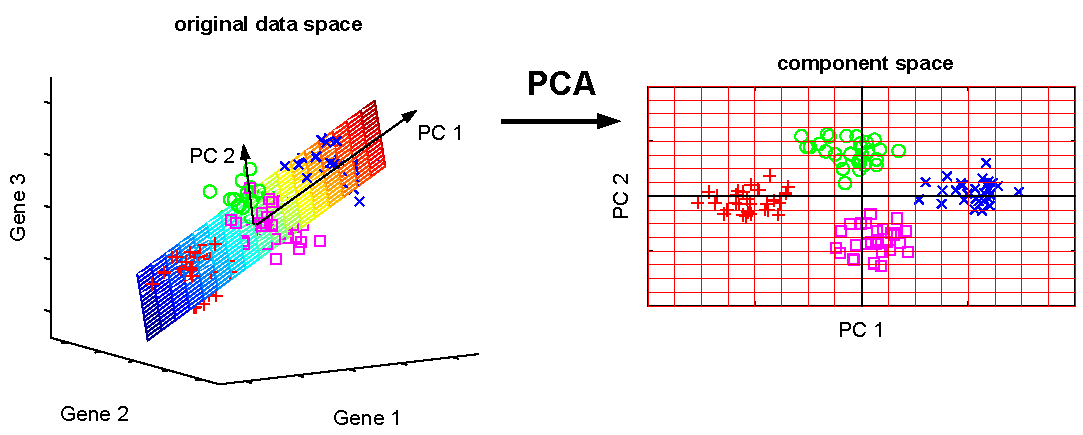
\includegraphics[width=0.47\textwidth]{figures/dim_reduct/fig_pca_illu3d}
  }% Store largest image in a box

  \begin{subfigure}[b]{0.48\textwidth}\centering
    \usebox{\largestimage}
    \vspace{0.01cm}
  \caption{PCA}
  \label{fig:dim_reduct:PCA:illustration}
  \end{subfigure}
  ~
  \begin{subfigure}[b]{\wd\largestimage}\centering
    \raisebox{\dimexpr.5\ht\largestimage-.5\height}{% Adjust vertical height of smaller image
      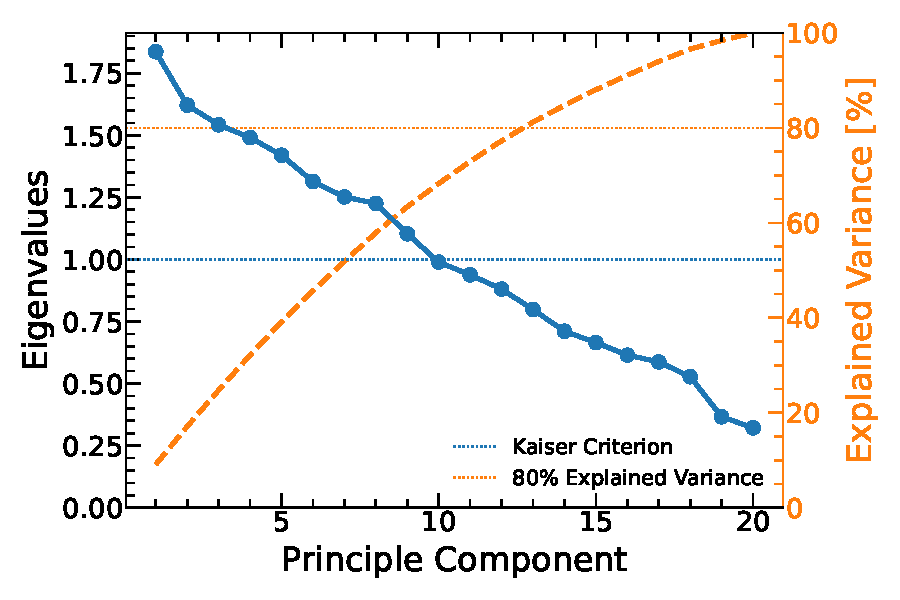
\includegraphics[width=\textwidth]{figures/dim_reduct/scree}}
  \caption{Scree Plot}
  \label{fig:dim_reduct:PCA:scree}
  \end{subfigure}
\caption{
On the left, an illustration of dimensionality reduction $m=3 \to k=2$ with PCA on genetics data \cite{Scholz2006}.
On the right, an example Scree plot from a toy dataset.
Based on these results we should consider reducing to $k=9$ or $13$ dimensions.
\label{fig:dim_reduct:PCA}
}
\end{figure}

%%%%%%%%%%%%%%%%%%%%%%%%%%%%%%%%%%%%%%%%%%%%%%%%%%%%%%%%
\subsection{Scree Plots}
\label{dim_reduct:PCA:Scree}
% TODO

% TODO Biplot?

TODO \cref{fig:dim_reduct:PCA:scree}

%%%%%%%%%%%%%%%%%%%%%%%%%%%%%%%%%%%%%%%%%%%%%%%%%%%%%%%%
%%%%%%%%%%%%%%%%%%%%%%%%%%%%%%%%%%%%%%%%%%%%%%%%%%%%%%%%
\section{Singular Value Decomposition (SVD)}
\label{dim_reduct:SVD}
% TODO

%%%%%%%%%%%%%%%%%%%%%%%%%%%%%%%%%%%%%%%%%%%%%%%%%%%%%%%%
%%%%%%%%%%%%%%%%%%%%%%%%%%%%%%%%%%%%%%%%%%%%%%%%%%%%%%%%
\section{Linear Discriminant Analysis (LDA)}
\label{dim_reduct:LDA}
% TODO

% TODO include Gaussian Discriminant Analysis (GDA) and Quadratic Discriminant Analysis (QDA)

%%%%%%%%%%%%%%%%%%%%%%%%%%%%%%%%%%%%%%%%%%%%%%%%%%%%%%%%
%%%%%%%%%%%%%%%%%%%%%%%%%%%%%%%%%%%%%%%%%%%%%%%%%%%%%%%%
\section{Isomap}
\label{dim_reduct:isomap}
% TODO

%%%%%%%%%%%%%%%%%%%%%%%%%%%%%%%%%%%%%%%%%%%%%%%%%%%%%%%%
%%%%%%%%%%%%%%%%%%%%%%%%%%%%%%%%%%%%%%%%%%%%%%%%%%%%%%%%
\section{Factor Analysis and Confounding Variables}
\label{dim_reduct:factor_ana}
% TODO

%%%%%%%%%%%%%%%%%%%%%%%%%%%%%%%%%%%%%%%%%%%%%%%%%%%%%%%%
%%%%%%%%%%%%%%%%%%%%%%%%%%%%%%%%%%%%%%%%%%%%%%%%%%%%%%%%
\section{Mutual Information (MI)}
\label{dim_reduct:MI}
% TODO

%%%%%%%%%%%%%%%%%%%%%%%%%%%%%%%%%%%%%%%%%%%%%%%%%%%%%%%%
\subsection{Normalized Mutual Information (NMI)}
\label{dim_reduct:MI:normalized}
% TODO

%%%%%%%%%%%%%%%%%%%%%%%%%%%%%%%%%%%%%%%%%%%%%%%%%%%%%%%%
%%%%%%%%%%%%%%%%%%%%%%%%%%%%%%%%%%%%%%%%%%%%%%%%%%%%%%%%
\section{Term Frequency-Inverse Document Frequency (TF-IDF)}
\label{dim_reduct:tfidf}

Term frequency-inverse document frequency (TF-IDF) is a statistic
used in natural language processing (NLP) to quantify
the importance, or uniqueness, of a term $t$ in a document $d$
with respect to a wider set of documents $D$\footnote{Note that $d$ is not necessarily an element of $D$, we can compare novel $d$ to a reference corpus $D$.}.
As the name suggests, TF-IDF is the product of two components,
one representing the frequency of the term under consideration within the document of interest,
and the other the inverse of the frequency of the term in all documents of the broader corpus.
There are a handful of definitions available for each term, but we will only describe
one of the more standard forms in this section:

\begin{subequations}\label{eq:unsupervised:tfidf}
\begin{align}
\text{tf}\left(t,d\right) &= \frac{n_{t,d}}{\sum_{t' \in d} n_{t',d}}, \label{eq:unsupervised:tfidf:tf} \\
\text{idf}\left(t,D\right) &= \log\left(\frac{\abs{D}}{1 + \abs{\left\{d' \in D \, | \, t \in d'\right\}}}\right), \label{eq:unsupervised:tfidf:idf} \\
\text{tf-idf}\left(t,d\right) &= \text{tf}\left(t,d\right) \times \text{idf}\left(t,D\right). \label{eq:unsupervised:tfidf:tfidf}
\end{align}
\end{subequations}

\noindent Here $n_{t,d}$ is number of times $t$ appears in $d$,
$\abs{D}$ is the number of documents in $D$,
and $\abs{\left\{d \in D \, | \, t \in d\right\}}$ is the number of number of documents in $D$ which contain $t$.
We take the natural log in the $\text{idf}\left(t,D\right)$ component to better accommodate large corpora of documents,
and include the constant $1+$ term to avoid divide-by-zero issues.

%%%%%%%%%%%%%%%%%%%%%%%%%%%%%%%%%%%%%%%%%%%%%%%%%%%%%%%%
%%%%%%%%%%%%%%%%%%%%%%%%%%%%%%%%%%%%%%%%%%%%%%%%%%%%%%%%
\section{Prevalence Ratio}
\label{dim_reduct:prevalence_ratio}

The prevalence ratio (PR) is a similar concept to TF-IDF,
allowing us to identify important characteristics of a population of interest versus the wider population.
For example, we can use a PR to assess the association of hypertension with heart failure by comparing
the prevalence of hypertension in a cohort of heart failure patients
to the prevalence of hypertension in the general population,
or at least a representative sample\footnote{Defining an acceptable representative sample is often the hardest part of the analysis and may require stratification, \eg stratifying by age when investigating disease.} of it.

The prevalence of a characteristic $c$ in a population $P$ is $\abs{\{p' \in P \, | \, c \in p'\}} \, / \, \abs{p' \in P}$,
note the similarity to $\text{tf}\left(t,d\right)$ \cref{eq:unsupervised:tfidf:tf}.
The prevalence ratio is then

\begin{equation}\label{eq:unsupervised:PR}
\text{PR}\left(t,d\right) = \frac{ \abs{\{p' \in P \, | \, c \in p'\}} \, / \, \abs{p' \in P} }{ \abs{\{p' \in P_{0} \, | \, c \in p'\}} \, / \, \abs{p' \in P_{0}} },
\end{equation}

\noindent where $P$ is the population of interest and $P_{0}$ is the wider population.

Note that the PR is mathematically identical to the relative risk, or hazard ratio (HR) discussed in \cref{chap:survival}.
There is a similar discussion in the literature \cite{pmid27460748,10.3389/fvets.2017.00193}
on prevalence ratios versus odds ratios as is described in \cref{survival:additional:odds}.

% See also: https://sph.unc.edu/wp-content/uploads/sites/112/2015/07/nciph_ERIC8.pdf

%%%%%%%%%%%%%%%%%%%%%%%%%%%%%%%%%%%%%%%%%%%%%%%%%%%%%%%%
%%%%%%%%%%%%%%%%%%%%%%%%%%%%%%%%%%%%%%%%%%%%%%%%%%%%%%%%
\section{\texorpdfstring{$t$}{t}-Distributed Stochastic Neighbor Embedding (\texorpdfstring{$t$}{t}-SNE)}
\label{dim_reduct:tSNE}
% TODO
% TODO \tSNE
